
\PassOptionsToPackage{table}{xcolor}

\documentclass[utf8]{beamer}

\usepackage[T1]{fontenc}
\usepackage[francais]{babel}
\usepackage{listings}
\usepackage{multicol}
\usepackage{tikz}
\usepackage{bibentry}

\setbeamertemplate{bibliography item}[text]
\setbeamertemplate{navigation symbols}{}
\usetheme{Amsterdam}

\usetikzlibrary{calc}
\tikzstyle{item}=[rectangle,rounded corners=3pt,thick, dashed, color=beamer@blendedgreen, fill=gray!20]
% Romain
\newcommand{\cRM}[1]{\MakeUppercase{\romannumeral #1}}  % Capital
\newcommand{\cRm}[1]{\textsc{\romannumeral #1}} % Petit majuscule
\newcommand{\crm}[1]{\romannumeral #1}
% Siècle %
\newcommand{\siecle}[1]{\cRM{#1}\textsuperscript{e}~siècle}

\definecolor{keywords}{RGB}{255,0,0}
\lstset{language=[LaTeX]TeX,
texcsstyle=*\color{keywords},
breaklines=true,
keywordstyle=\color{keywords},
commentstyle=\color{darkgreen},
tabsize=2,
backgroundcolor=\color{lightgrey},
escapeinside=||,
morekeywords={*,subsection,make title,tableofcontents,include graphics}
}


\definecolor{lightgrey}{rgb}{0.9,0.9,0.9}
\definecolor{darkgreen}{rgb}{0,0.6,0} 
\rowcolors{1}{gray!25}{white}

\title{L'intégration des technologies de l'information dans l'éducation}
\author{Chloé DESDOUITS, William DYCE, Thibaut MARMIN, Clément SIPIETER}
\date{\today}

\AtBeginSection[]{
  \begin{frame}[plain]
  	\frametitle{Sommaire}
  	\tableofcontents[currentsection]
  \end{frame} 
}

\begin{document}

\frame[plain]{\titlepage}

\begin{frame}[plain]
	\frametitle{Sommaire}
	\tableofcontents
\end{frame} 



\section{Intégration des TIC\ldots}

\subsection{\ldots dans l'éducation}

\begin{frame}{test}
test
\end{frame}

\subsection{\ldots dans la société}

\begin{frame}{test}
test
\end{frame}



\section{Évolutions divergentes}

\subsection{Des formations en inadéquation avec les besoins des entreprises}

\begin{frame}{test}
\begin{tikzpicture}[remember picture,overlay]
	\node[anchor=south east,inner sep=0pt] at ($(current page.south east)+(-1.35cm,0.4cm)$) {
		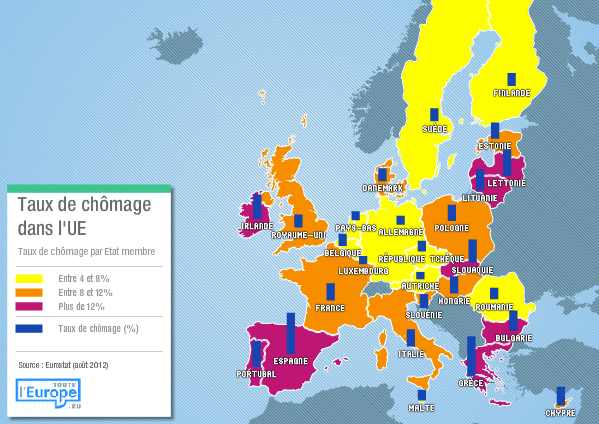
\includegraphics[trim=0cm 0cm 0cm 0cm, clip=true, scale=0.31]{../figures/chom}
	};
\end{tikzpicture}
\footlineextra{\cite{portables40}}
\end{frame}

\subsection{Les retombées imprévues de l'utilisation des technologies de la communication}

\begin{frame}{test}
test
\end{frame}

\subsection{Décrochages et échecs scolaires}

\begin{frame}{test}
test
\end{frame}



\section{Solutions}

\subsection{Initiatives des pouvoirs publics}

\begin{frame}{test}
test
\end{frame}

\subsection{Initiatives d'autres acteurs}

\begin{frame}{test}
test
\end{frame}

\subsection{Quelles peuvent être les solutions adaptées pour endiguer le phénomène ?}

\begin{frame}{test}
test
\end{frame}



\section{Bibliographie}
\bibliographystyle{plain}
\begin{frame}[allowframebreaks]
\frametitle{Bibliographie}
\bibliography{../Bib.bib}
\end{frame}

\end{document}


